\documentclass{beamer}
\mode<presentation>
\usetheme{Boadilla}

\usepackage{amsmath,amssymb}
\usepackage{graphicx}
\usepackage{siunitx}
\sisetup{per-mode=symbol}
\usepackage{gvv}
\usepackage{listings}
\usepackage{xcolor}

% Code style
\lstset{
  basicstyle=\ttfamily\scriptsize,
  breaklines=true,
  frame=single,
  numbers=left,
  numberstyle=\tiny,
  keywordstyle=\color{blue},
  commentstyle=\color{green!50!black},
  stringstyle=\color{red!60!black},
  showstringspaces=false
}

\title{Matrix 2.6.24}
\author{ai25btech11015 -- M Sai Rithik}
\date{}


\begin{document}
\frame{\titlepage}

\begin{frame}
\frametitle{Question (2.6.24)}
Find the area of the parallelogram whose adjacent sides are given by the vectors
\[
\Vec{a} = 3\hat{i} + \hat{j} + 4\hat{k}, \quad 
\Vec{b} = \hat{i} - \hat{j} + \hat{k}.
\]
Do not use determinant method; use $\|\Vec{a}\|\|\Vec{b}\|\sin\theta$.
\end{frame}

\begin{frame}
\frametitle{Step 1: Representing Vectors}
\begin{equation}
\Vec{a} = \myvec{3 \\ 1 \\ 4}, \qquad
\Vec{b} = \myvec{1 \\ -1 \\ 1}.
\end{equation}
\end{frame}

\begin{frame}
\frametitle{Step 2: Magnitudes}
\begin{equation}
\|\Vec{a}\| = \sqrt{3^2 + 1^2 + 4^2} = \sqrt{26},
\end{equation}
\begin{equation}
\|\Vec{b}\| = \sqrt{1^2 + (-1)^2 + 1^2} = \sqrt{3}.
\end{equation}
\end{frame}

\begin{frame}
\frametitle{Step 3: Dot Product and $\cos\theta$}
\begin{equation}
\Vec{a}\cdot\Vec{b} = 3(1) + 1(-1) + 4(1) = 6,
\end{equation}
\begin{equation}
\cos\theta = \frac{\Vec{a}\cdot\Vec{b}}{\|\Vec{a}\|\|\Vec{b}\|}
= \frac{6}{\sqrt{26}\sqrt{3}} = \frac{6}{\sqrt{78}}.
\end{equation}
\end{frame}

\begin{frame}
\frametitle{Step 4: Finding $\sin\theta$}
\begin{equation}
\sin\theta = \sqrt{1 - \cos^2\theta}
= \sqrt{1 - \left(\frac{6}{\sqrt{78}}\right)^2},
\end{equation}
\begin{equation}
\sin\theta = \sqrt{\frac{7}{13}}.
\end{equation}
\end{frame}

\begin{frame}
\frametitle{Step 5: Area of Parallelogram}
\begin{equation}
\text{Area} = \|\Vec{a}\| \|\Vec{b}\| \sin\theta,
\end{equation}
\begin{equation}
= \sqrt{26}\,\sqrt{3}\,\sqrt{\tfrac{7}{13}}
= \sqrt{42}.
\end{equation}
\end{frame}

\begin{frame}
\frametitle{Final Answer}
\begin{equation}
\boxed{\text{Area} = \sqrt{42}}
\end{equation}
\begin{figure}[h!]
    \centering
    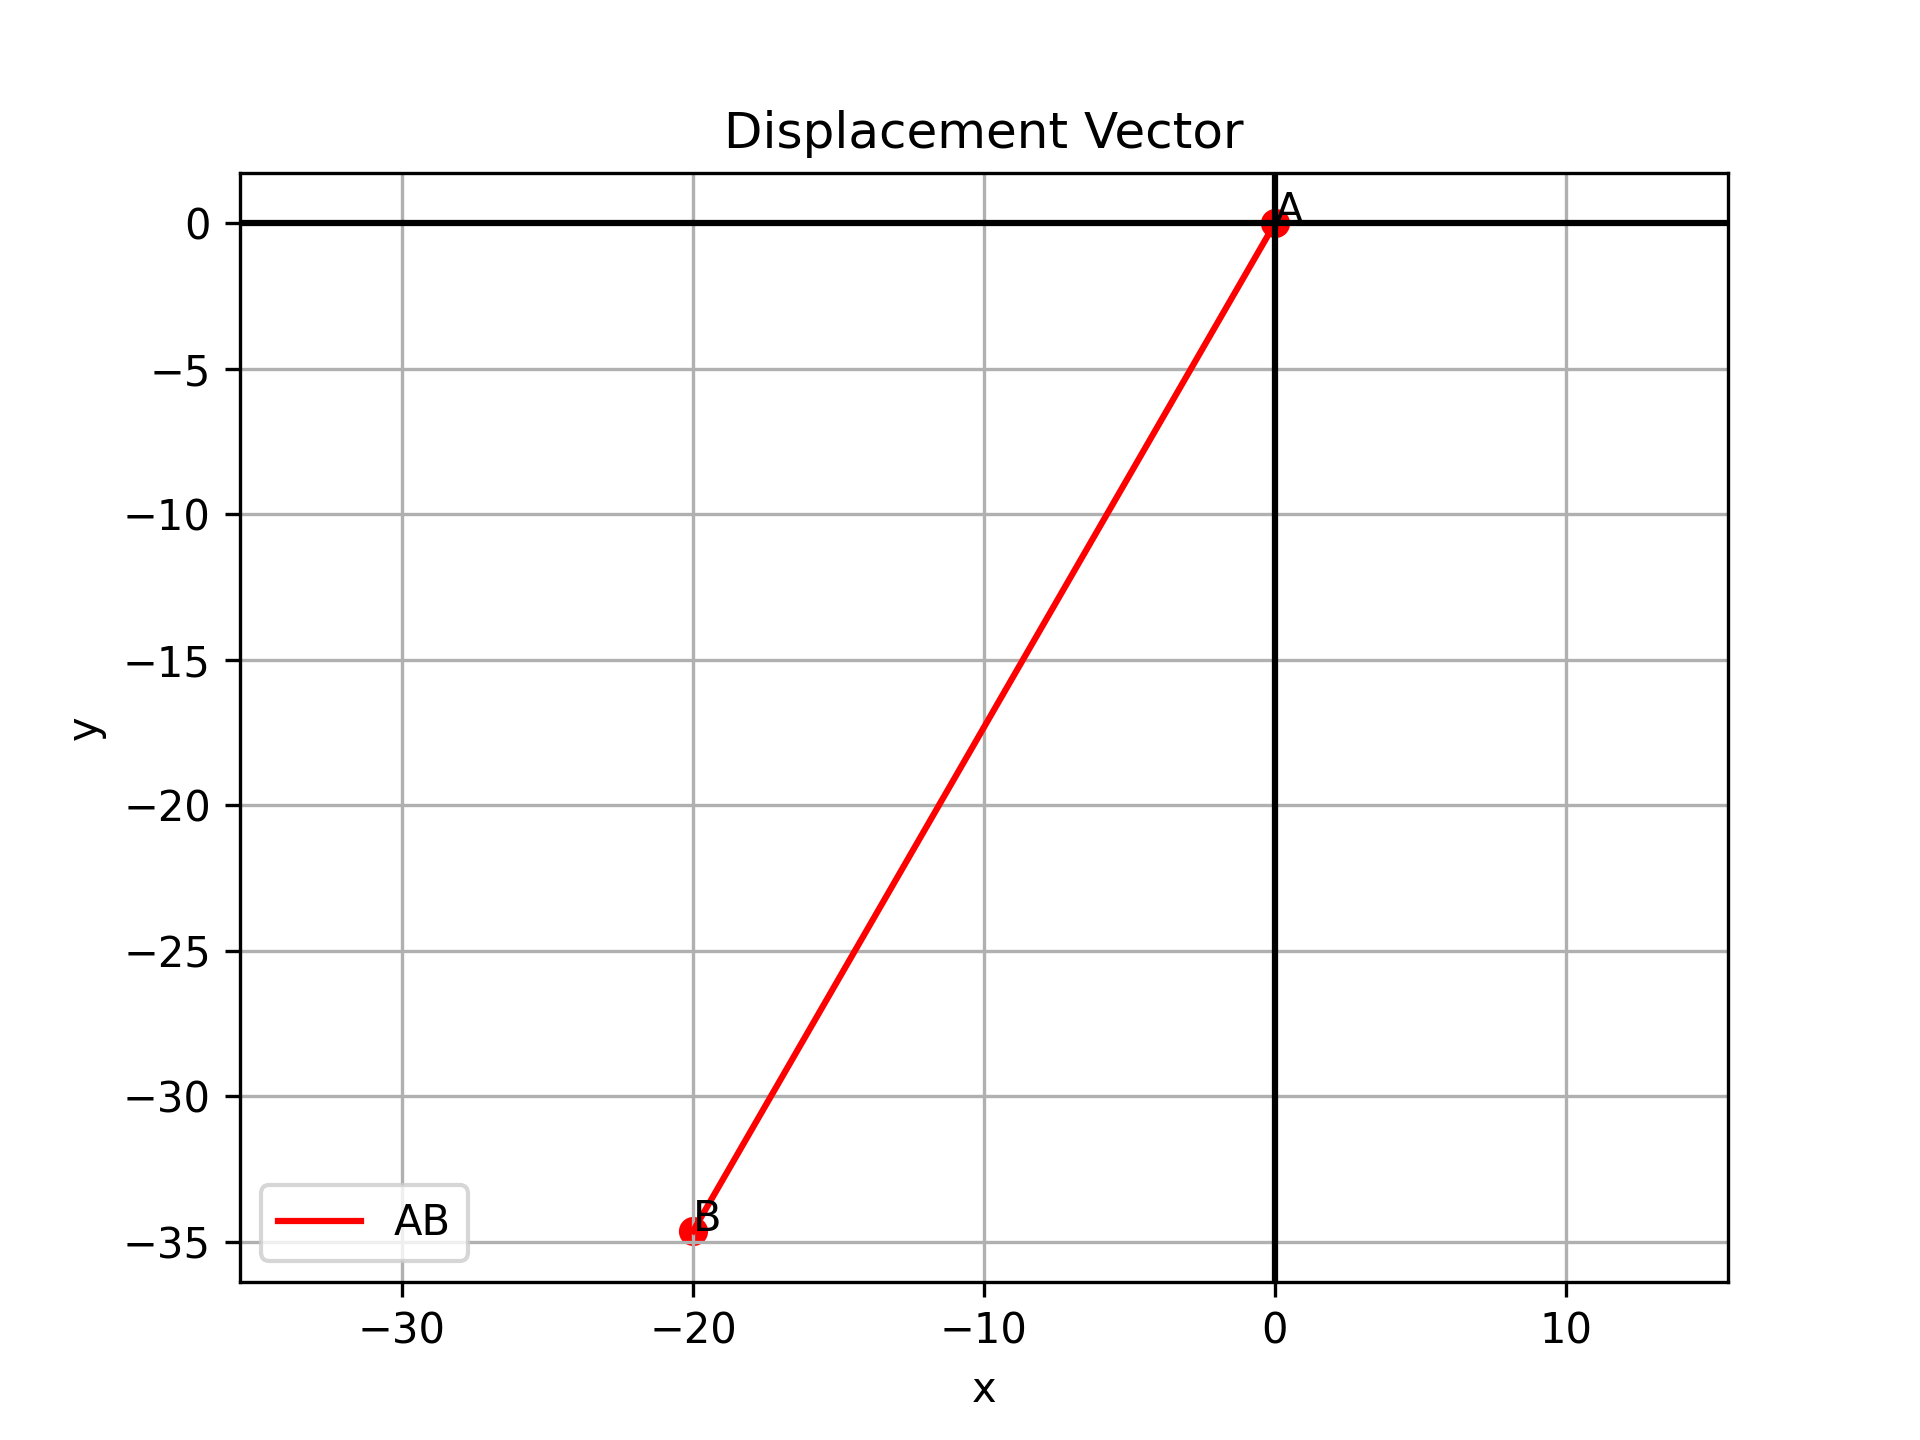
\includegraphics[width=0.6\linewidth]{figs/fig.png}
    \caption{Parallelogram spanned by $\Vec{a}$ and $\Vec{b}$.}
\end{figure}
\end{frame}

\begin{frame}[fragile]
    \frametitle{C Code}
    \begin{lstlisting}[language=C]
// C code to calculate area of parallelogram
#include <stdio.h>
#include "libs/matfun.h"
#include <math.h>

int main() {
    // create a b vectros 
    double **a = createMat(3,1);
    a[0][0] = 3;
    a[1][0] = 1;
    a[2][0] = 4;

    double **b = createMat(3,1);
    b[0][0] = 1;
    b[1][0] = -1;
    b[2][0] = 1;

\end{lstlisting}
\end{frame}

\begin{frame}[fragile]
    \frametitle{C Code}
    \begin{lstlisting}[language=C]
    double mag_a = sqrt(Matdot(a, a,3));
    double mag_b = sqrt(Matdot(b, b,3));

    double cos_theta = Matdot(a, b,3) / (mag_a * mag_b);
    double angle = acos(cos_theta);

    double area = mag_a * mag_b * sin(angle);

    FILE *fp = fopen("var.dat", "w");
    if (fp != NULL) {
        fprintf(fp, "%lf\n", area);
        fclose(fp);
    } else {
        printf("Error opening file for writing.\n");
    }
    return 0;
}

\end{lstlisting}
\end{frame}

\begin{frame}[fragile]
    \frametitle{Python Code}
    \begin{lstlisting}[language=python]
import numpy as np 
from mpl_toolkits.mplot3d import Axes3D
from mpl_toolkits.mplot3d.art3d import Poly3DCollection
import matplotlib.pyplot as plt
with open('var.dat', 'r') as f:
	area = f.read().strip()

a = np.array([3, 1, 4])
b = np.array([1, -1, 1])
O = np.array([0, 0, 0])

fig = plt.figure()
ax = fig.add_subplot(111, projection='3d')

# Plot vectors OA and OB
ax.quiver(*O, *a, color='r', label='OA')
ax.quiver(*O, *b, color='b', label='OB')
ax.text(a[0], a[1], a[2], 'OA', color='r', fontsize=12)
ax.text(b[0], b[1], b[2], 'OB', color='b', fontsize=12)

verts = [ [O, a, a+b, b] ]
ax.add_collection3d(Poly3DCollection(verts, alpha=0.3, facecolor='green'))
\end{lstlisting}
\end{frame}

\begin{frame}[fragile]
    \frametitle{Python Code}
    \begin{lstlisting}[language=C]

# Set limits and labels
ax.set_xlim([0, max(a[0], b[0], a[0]+b[0])+1])
ax.set_ylim([min(0, a[1], b[1], a[1]+b[1])-1, max(a[1], b[1], a[1]+b[1])+1])
ax.set_zlim([0, max(a[2], b[2], a[2]+b[2])+1])
ax.set_xlabel('X')
ax.set_ylabel('Y')
ax.set_zlabel('Z')
ax.legend()

# Set the graph title to the area value
ax.set_title(f'Area = {area}')

plt.tight_layout()
plt.savefig('../figs/vectors_3d.png')
plt.close()

\end{lstlisting}
\end{frame}
\end{document}
